%Publication version
%\documentclass[aps,twocolumn,prd,superscriptaddress,showpacs,nofootinbib,fixfloat]{revtex4}
%Draft version
\documentclass[aps,prd,superscriptaddress,showpacs]{revtex4}
%\usepackage{doublespace}
\usepackage{graphicx}
\usepackage{dcolumn}
\usepackage{bm}
\usepackage{natbib}

%\topmargin+1cm

\hyphenation{CTBCORE}

% Journals
\newcommand{\aaps}{{Astron.~Astrophys.~Supp.}}
\newcommand{\physrep}{{Physics~Reports}}
\newcommand{\araa}{{Annu.~Rev.~Astron.~Astrophys.}}
\newcommand{\aap}{{Astron.~Astrophys.}}
\newcommand{\apjl}{{Astrophys.~J.~Lett.}}
\newcommand{\apjs}{{Astrophys.~J.~Supp.}}
\newcommand{\aj}{{Astron.~J.}}
\newcommand{\mnras}{{Mon.~Not.~R.~Astron.~Soc.}}

% Making life easier
\newcommand{\be}{\begin{equation}}
\newcommand{\ee}{\end{equation}}
\newcommand{\bea}{\begin{eqnarray}}
\newcommand{\eea}{\end{eqnarray}}
\newcommand{\backten}{\!\!\!\!\!\!\!\!\!\!}

% useful symbols
\newcommand{\nhat}{\hat{\bf n}}
\newcommand{\kvec}{{\bf k}}
\newcommand{\edm}{\epsilon_{dm}}
\newcommand{\edmnow}{\epsilon_{dm,0}}
\newcommand{\sv}{\langle\sigma_Av\rangle}
\newcommand{\khat}{\hat{\bf k}}

% Fermi is usually italicized - use \Fermi\ for space after word
\newcommand{\Fermi}{{\slshape Fermi}}

% math functions, units
\newcommand{\Mpc}{{\rm ~Mpc}}
\newcommand{\sech}{{\rm ~sech~}}
\newcommand{\Tr}{{\rm ~Tr~}}
\newcommand{\threej}[6]{{\left( \begin{array}{ccc} #1 & #2 & #3 \\ #4 & 
   #5 & #6 \end{array} \right)}}

% Doug's units
\newcommand{\s}{{\rm ~s}}
\newcommand{\kms}{{\rm ~km/s}}
\newcommand{\g}{{\rm ~g}}
\newcommand{\cm}{{\rm ~cm}}
\newcommand{\ph}{{\rm ~ph}}
\newcommand{\sr}{{\rm ~sr}}
\newcommand{\km}{{\rm ~km}}
\newcommand{\mm}{{\rm ~mm}}
\newcommand{\mJy}{{\rm ~mJy}}
\newcommand{\Jy}{{\rm ~Jy}}
\newcommand{\MJy}{{\rm ~MJy}}
\newcommand{\MJypSr}{{\rm ~MJy~sr^{-1}}}
\newcommand{\JypSr}{{\rm ~Jy~sr^{-1}}}
\newcommand{\Hz}{{\rm ~Hz}}
\newcommand{\kHz}{{\rm ~kHz}}
\newcommand{\MHz}{{\rm ~MHz}}
\newcommand{\GHz}{{\rm ~GHz}}
\newcommand{\K}{{\rm ~K}}
\newcommand{\mK}{\rm ~mK}
\newcommand{\microK}{\mu{\rm K}}
\newcommand{\eV}{{\rm ~eV}}
\newcommand{\eVs}{{\rm ~eV/s}}
\newcommand{\keV}{{\rm ~keV}}
\newcommand{\MeV}{{\rm ~MeV}}
\newcommand{\GeV}{{\rm ~GeV}}
\newcommand{\TeV}{{\rm ~TeV}}
\newcommand{\pc}{{\rm ~pc}}
\newcommand{\kpc}{{\rm ~kpc}}
%\newcommand{\Mpc}{{\rm ~Mpc}}
\newcommand{\erg}{{\rm ~erg}}
\newcommand{\degree}{^{\rm o}}
\newcommand{\sigmav}{\langle\sigma_Av\rangle}
\newcommand{\zrock}{$Z_{\rm rock}$}
\newcommand\reftbl[1]{Table \ref{tbl:#1}}
\def\la{\vcenter{\hbox{$<$}\offinterlineskip\hbox{$\sim$}}}
\def\ga{\vcenter{\hbox{$>$}\offinterlineskip\hbox{$\sim$}}}
\newcommand\Refsec[1]{Section \ref{sec:#1}}

% Necessary for appendices

%% \newcommand\dpf[1]{{\bf (DPF: #1)}}
%% \newcommand\dpf[1]{{\bf (MS: #1)}}
%% \newcommand\dpf[1]{{\bf (CW: #1)}}

\begin{document}


\title{Fermi White Paper}

\author{Douglas P. Finkbeiner}
%\email{dfinkbeiner@cfa.harvard.edu}
\affiliation{Institute for Theory and Computation,
  Harvard-Smithsonian Center for Astrophysics, 
  60 Garden Street, MS-51, Cambridge, MA 02138, USA} 
\affiliation{Center for the Fundamental Laws of Nature,
  Physics Department, 
  Harvard University, 
  Cambridge, MA 02138 USA}

\author{Meng Su}
\affiliation{Institute for Theory and Computation,
  Harvard-Smithsonian Center for Astrophysics, 
  60 Garden Street, MS-51, Cambridge, MA 02138, USA} 
\affiliation{Department of Physics, and Kavli Institute for Astrophysics and Space Research, Massachusetts Institute of Technology, Cambridge, MA 02139, USA}
\affiliation{Einstein Fellow}

\author{Christoph Weniger}
\affiliation{Amsterdam}

\author{Nestor Mirabel}
\affiliation{affil}

%% Claims of a line are important and demand a careful search for
%% systematics.  Limb photons provide a reference spectrum and look a bit
%% fishy.  Need more data.
\begin{abstract} Does a white paper have an abstract?
\end{abstract}

\pacs{95.35.+d}

\maketitle


%%%%%%%%%%%%%%%%%%%%%% SECTION I %%%%%%%%%%%%%%%%%%%%%%%%%%%%%%%

\section{Introduction}


The search for non-gravitational signatures from WIMP
(weakly interacting massive particle) dark matter has 
generally been approached from three different directions: missing
energy searches at colliders, direct searches for the
recoil of nuclei from underground detectors, and indirect
methods including searching for dark matter signals from cosmic
rays (CR) and multiwavelength astronomical
observations~\citep{Jungman:1995df, Bergstrom:2000, Bertone:2005, Hooper:2007Review,
2012arXiv1205.4882B, Cirelli:2012tf}.

For indirect detection, distinguishing the dark matter
signal from conventional astrophysical backgrounds is
challenging
(for a recent review on indirect searches with gamma rays
see~\cite{Bringmann:2012ez}).
Among various possible signatures, gamma-ray
line emission is a long-sought ``smoking
gun'' for dark matter annihilation~\cite{Bergstrom:1988fp}, as no plausible
astrophysical background can produce such a line
signature.\footnote{A narrow feature is
possible in theory~\citep[see][]{2012arXiv1207.0458A}.}  Gamma-ray line(s)
could be produced by dark matter decays or annihilations
into two photons, or two-body final states involving one
photon plus a Higgs boson, Z boson, or other neutral non-SM
particle.  In most models, the branching ratio
to lines is loop suppressed relative to the continuum
emission, and one would have expected to see the continuum
first in e.g. MSSM models~\citep[e.g.][]{Bergstrom:1997}.
Although this theoretical prejudice led most previous
studies to focus on continuum searches, there are models
being proposed that allow high line to continuum
ratios~\citep[e.g.][]{Bergstrom:1998, Bergstrom:2000,
Bertone:2009, Jackson:2010, Cline:2012, Weiner:2012}.
However, previous searches in EGRET~\cite{Pullen:2006sy} and \Fermi-LAT
data~\cite{Abdo:2010nc, Vertongen:2011mu, Ackermann:2012qk}
did not find any
indications for a gamma-ray line signal and presented only upper limits on the
line flux.

The first claims for a spectral feature around 130 GeV were made by Bringmann
\textit{et al.}~\citep{Bringmann:2012} and Weniger~\citep{Weniger:2012}. While
Ref.~\citep{Bringmann:2012} mostly concentrated on an interpretation in the context of
virtual internal Bremsstrahlung signals from annihilations,
Ref.~\citep{Weniger:2012} focused on gamma-ray lines and a thorough discussion
of possible instrumental effects.  Both works performed a spectral fit to
photon events in regions of interest in
the inner Galaxy designed to maximize S/N. The significance of the line structure
at 130 GeV was found to be 4.6$\sigma$, or 3.2$\sigma$ after the trials factor
correction~\citep{Weniger:2012}.
This claim was quickly followed up and disputed by a number of
groups~\cite{tempel:2012ey, Boyarsky:2012ca}.

Subsequent work by Su \& Finkbeiner approached the problem
with template fitting, which takes into account the spatial
distribution of events along with spectral information,
assuming various profiles (Einasto, NFW, Gaussian) for the
DM distribution~\citep{linepaper}.  If the template is
correct, this allows extraction of the DM signal with higher
S/N.  This work found 6.6$\sigma$ (5.1$\sigma$ after the
trials factor correction) for an Einasto profile centered
$1.5\degree$ west of the Galactic center, and also suggested
that there may be two lines, at about 111 and 129 GeV.  The
lower energy line is tantalizing because it matches the
expected energy of a $Z\gamma$ line if the higher energy is
the $\gamma\gamma$ line.  These findings have inspired a
number of models and further analysis of the \Fermi\
data~\citep{Dudas:2012, Choi:2012, Kyae:2012, Lee:2012,
Rajaraman:2012, Acharya:2012, Garny:2012, Buckley:2012,
Chu:2012, Kang:2012, Buchmuller:2012, Bergstrom:2012b,
Heo:2012, Park:2012, Tulin:2012, Cline:2012, Weiner:2012,
WeinerYavin:2012b, FanReece:2012, Huang:2012, Whiteson:2012,
Buchmuller:2012, Cholis:2012}.

Recent evidence for lines at 111 GeV and 129 GeV with a
local significance of $3.3\sigma$ from \Fermi\ unassociated
point sources suggests an annihilation signal is
present~\cite{doubleline}\citep[but
see][]{HooperLinden:2012b}, as does the claim of line
emission from galaxy clusters at 130
GeV~\cite{Hektor:2012kc}.  Neither of these would stand on
their own, but they provide support for the hypothesis that
the Galactic center line signal is produced by dark matter
annihilation.

The high statistical significance of the line feature
motivates a search for systematic errors in the LAT data
that could mimic a line in the Galactic center.
Confirmation by Imaging Air Cherenkov Telescopes like
HESS-II might be possible as early as next
year~\cite{Bergstrom:2012}, but in the meantime a thorough
study of LAT systematics is urgently needed.  We do not have
access to the details of the reconstruction of each photon
event, which would allow us to study how it developed in the
tracker and calorimeter.  However, we do have information
about each event from the public event lists and spacecraft
parameter files.  We can use this information to search for
any line-producing artifacts in the detector frame, and
investigate if they could map onto the Galactic center.

The Earth's atmosphere provides a convenient source of
photons for systematics tests.  The continual cosmic-ray
cascades in the Earth's atmosphere produce gamma rays with
$dN/dE \sim E^{-2.8}$~\citep{FermiLimb}.  Because these
so-called `Earth limb photons' result from atmospheric
cascades, they are produced by interactions in a highly
boosted frame, and cannot contain line emission.
\medskip


\begin{figure}[h]
  \begin{center}
    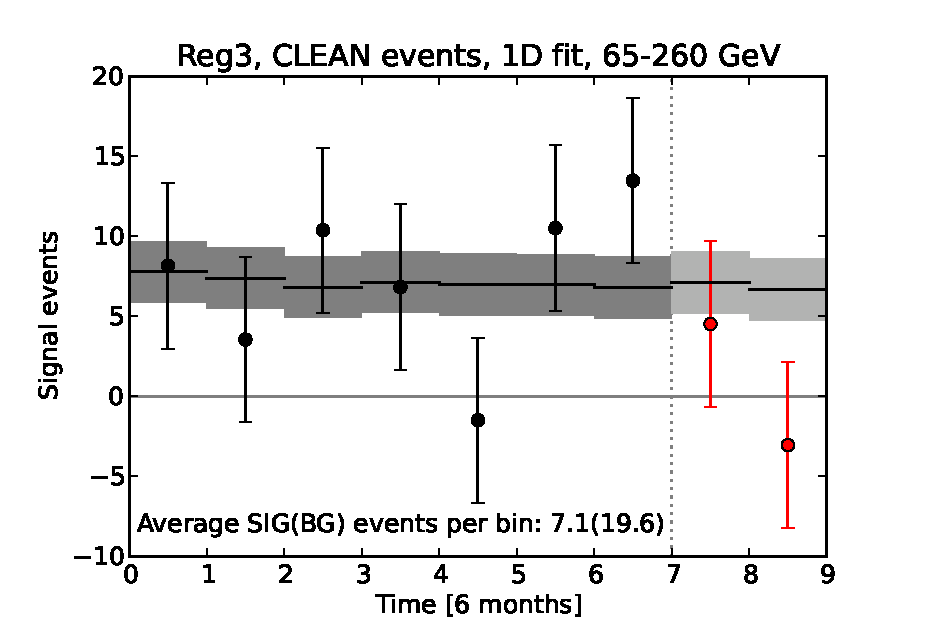
\includegraphics[width=0.66\linewidth]{plots/semester_fluxes.eps}
    \vspace{-0.5cm}
  \end{center}
  \caption{Number of signal events measured in 6-month intervals since 4
    August 2008, as obtained by an unbinned likelihood fit to the data in
    Region 3 ???. The average number of signal (background) events in the first
    3.5 years is 1.0 (2.4) per month. In red we show data taken since 4
    February 2012.}
  \label{fig:semester_fluxes}
\end{figure}


\begin{figure}[h]
  \begin{center}
    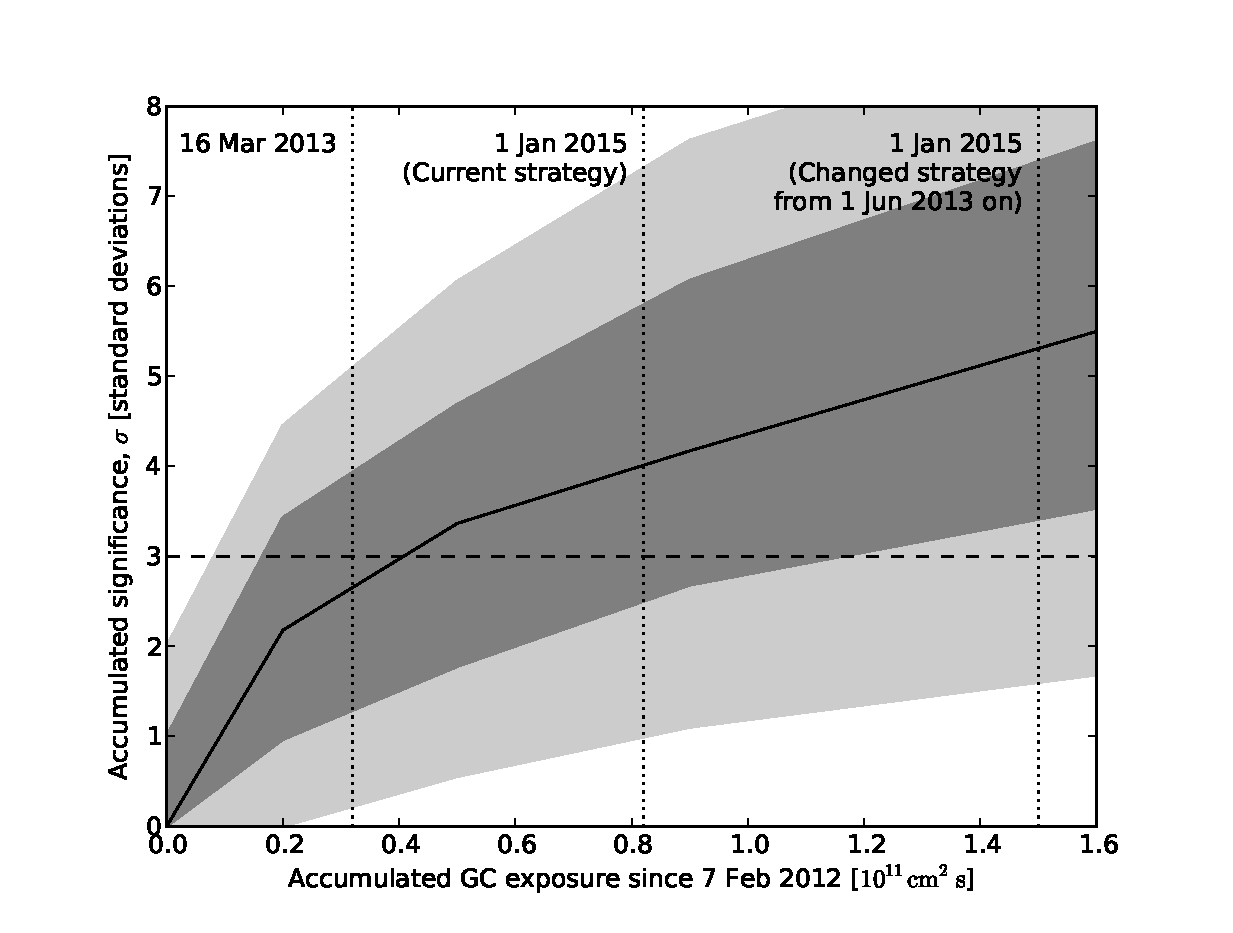
\includegraphics[width=0.8\linewidth]{plots/projection.eps}
    \vspace{-0.5cm}
  \end{center}
  \caption{Evaluation of mixed observation strategy. \emph{Top panel:}
    Effective energy resolution in different sky regions. \emph{Central
      panel:} change in exposure relative to standard survey
    mode. \emph{Bottom panel:} Figure of merit for gamma-ray line searches in
    different sky regions.}
  \label{fig:option}
\end{figure}


\begin{figure}[h]
  \begin{center}
    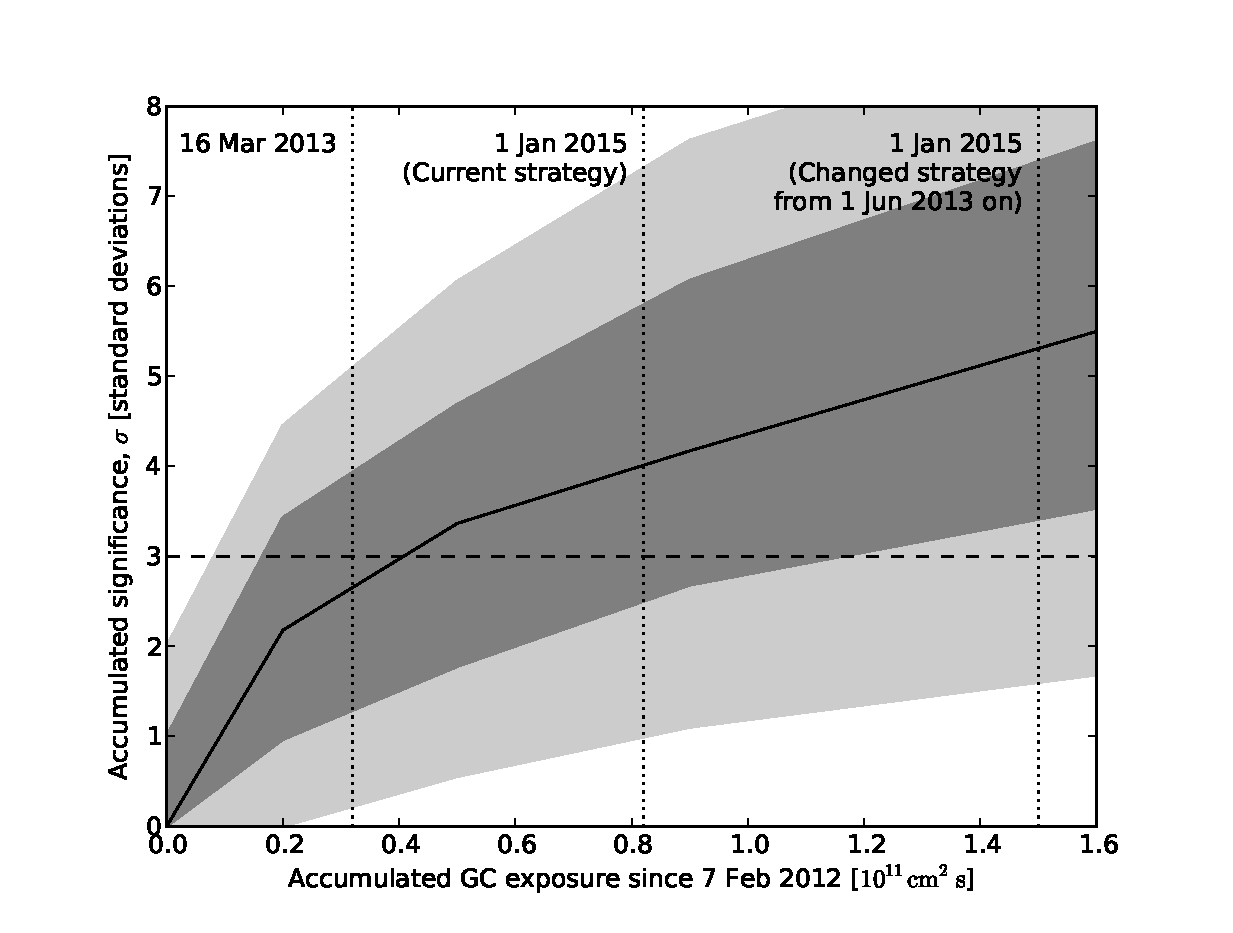
\includegraphics[width=0.8\linewidth]{plots/projection.eps}
    \vspace{-0.5cm}
  \end{center}
  \caption{Expected growth in signal significance as new data are accumulated,
    starting from 7 February 2012. The shaded bands show $68\%$ and $95\%$
    C.L., and are derived from a Monte Carlo simulation. For the predictions,
    we adopt the signal and background fluxes as they were measured prior to 7
    February 2012. The second and third vertical dotted lines indicate
    respectively the accumulated exposure until end of 2014 when the
    observation strategy remains unchanged, and when the mixed observation
    strategy is adopted starting from June 2013 (see Fig. 2)}
  \label{fig:projection}
\end{figure}




\section{Discussion and Conclusion}
\label{sec:Conclusion}

In this white paper we have argued for a change in the Fermi strategy on the
following basis.


\begin{itemize}

\item{\bf It is important: discovery of a dark matter annihilation line in the
    Galactic center would be Fermi's greatest accomplishment.}  The nature of
  dark matter is one of the greatest mysteries in physics and astrophysics,
  and the disovery of a line would be a major step forward for both fields.
  Exploring the nature of dark matter is one of the major goals of the Fermi
  project, and a discovery would define Fermi's legacy.

\item{\bf Fermi can do it: a modified survey strategy can obtain a decisive
    measurement, while the status quo cannot.}  I think that 2 years of
  altered survey mode are enough to get a definitive answer.  Calculations we
  have done with Weniger this week show that we need more exposure than I
  thought to get a definitive answer.  If we go with standard survey mode
  until 2016, there is a decent chance that we leave this question unresolved.
  We cannot permit that to happen.

\item{\bf A change is not bad for other science.}  There will be winners and
  losers in any change, but more time on the inner Galaxy is good for lots of
  projects (better time coverage for pulsars and transients, etc.) and it is
  not like we will never observe the rest of the sky.

\item{\bf It looks good for future funding.}  Enough said. 

\end{itemize}

Daniel Eisenstein was both eloquent and forceful about this last point
when we discussed it with him yesterday for an hour.  I'm not sure he
meant to be quoted, but the gist was that there are two possible
scenarios for the situation walking into the senior review:

1.  The LAT saw hints of something that could be its most important
discovery.  The project responded by a call for white papers, decided
to change strategy, and is now N months into a modified survey mode
with a promise of an answer at 99\% confidence by X date.
OR
2.  The LAT saw hints of something that could be its most important
discovery.  The project responded by a call for white papers, and then
did ... nothing.

He was pretty sure option 1 is better for continued funding.  He would
know, since he has done a lot of senior reviewing himself.  I know we
have all discussed this before, but he put it starkly enough to bring
it home.  The mistake we might make by doing this is not as bad as the
mistake of doing nothing and letting this opportunity slip by.

Daniel felt strongly (as have *all* the other colleagues I have
consulted) that we should do this, and as soon as possible.  So for
all of these reasons, I intended to be a strong advocate for making a
change.



\clearpage
\bibliography{whitepaper}

\end{document}
